\documentclass[12 pt, a4paper]{article}% тип документа, размер шрифта
\usepackage{cmap}	
\usepackage{hyperref}
\hypersetup{
	colorlinks=true,
	linkcolor=blue,
	urlcolor=blue,
}
\usepackage{mathtext}
\usepackage[T2A]{fontenc}%поддержка кириллицы в ЛаТеХ
\usepackage[utf8]{inputenc}%кодировка
\usepackage[english,russian]{babel}
\usepackage{indentfirst}

\usepackage{amsmath,amsfonts,amssymb,amsthm,mathtools} % AMS
\usepackage{amsmath}%удобная вёрстка многострочных формул, масштабирующийся текст в формулах, формулы в рамках и др.
\usepackage{amsfonts}%поддержка ажурного и готического шрифтов — например, для записи символа {\displaystyle \mathbb {R} } \mathbb {R} 
\usepackage{amssymb}%amsfonts + несколько сотен дополнительных математических символов
\frenchspacing%запрет длинного пробела после точки
\usepackage{setspace}%возможность установки межстрочного интервала
\usepackage{indentfirst}%пакет позволяет делать в первом абзаце после заголовка абзацный отступ
\onehalfspacing%установка полуторного интервала по умолчанию
\usepackage{graphicx}%подключение рисунков
\graphicspath{{images/}}%путь ко всем рисункам
\usepackage{caption}
\usepackage{float}%плавающие картинки
\usepackage{tikz} % это для чудо-миллиметровки
\usepackage[export]{adjustbox}
\usepackage{pgfplots}%для построения графиков
\pgfplotsset{compat=newest, y label style={rotate=-90},  width=10 cm}%версия пакета построения графиков, ширина графиков
\usepackage{pgfplotstable}%простое рисование табличек
\usepackage{lastpage}%пакет нумерации страниц
\usepackage{comment}%возможность вставлять большие комменты
\usepackage{float}
%%%%% ПОЛЯ
\setlength\parindent{0pt} 
\usepackage[top = 2 cm, bottom = 2 cm, left = 1.5 cm, right = 2 cm]{geometry}
\setlength\parindent{0pt}
%%%%% КОЛОНТИТУЛЫ
\usepackage[shortlabels]{enumitem}

\usepackage{array,tabularx,tabulary,booktabs} % Дополнительная работа с таблицами
\usepackage{longtable} % Длинные таблицы
\usepackage{multirow} % Слияние строк в таблице
\usepackage{colortbl} % Цветная заливка в таблице
\usepackage[labelsep=period,labelfont=rm,tablename={Таблица},tablewithin=none]{caption}
\usepackage{makecell} 
\usepackage{ctable} % for \specialrule command 

\usepackage{fancybox, fancyhdr}
\pagestyle{fancy} 
\fancyhead[L]{\textit{6 класс}}
\fancyhead[C]{\textit{{ЛМШ "Алые паруса" 2023}}}
\fancyhead[R]{\textit{2 день}} % ЛЮБАЯ ДОПОЛНИТЕЛЬНАЯ ИНФОРМАЦИЯ
%\fancyfoot[R]{Задание с двух сторон!}
\renewcommand{\footrulewidth}{0.3 mm}

\usepackage{tikzsymbols}
\usepackage{textcomp}
\usepackage{parskip}
\usepackage{graphicx}
\graphicspath{{pictures/}}
\DeclareGraphicsExtensions{.pdf,.png,.jpg}
\usepackage{wrapfig}
%%% Заголовок

%%% Новые команды
\newcommand{\z}[1]{{{\vspace{0.6cm} \large\textbf{{Задача {#1}} \\ }}}}
\newcommand{\task}[1]{{{\vspace{0.6cm} \vspace{-2ex} \textbf{№{#1}}  }}}
\newcommand{\otv}{{\vspace{0.3cm} \textbf{Решение: } \\}}
\newcommand{\uk}{\underline{\textit{Указание.}} }
\newcommand{\opr}{\textit{Определение: }}
\newcommand{\sol}[1]{{{\vspace{0.3cm} \textbf{{Задача {#1}} }\\ }}}
\newcommand{\RomanNumeralCaps}[1]
{\MakeUppercase{\romannumeral #1}}

\usepackage{cancel}
\usepackage{epigraph} 
\setlength\parindent{0pt}
\setlength\parskip{1ex plus 2pt minus 1pt}
\newcommand\X{\par\noindent---~}
\usepackage{ upgreek }
\begin{document} % конец преамбулы, начало документа
	\newpage
	\begin{flushright}
		\textit{<<Чёрт знает, чем всё кончится, но хорошо, что хоть начинается.>>}
	\end{flushright}
	\begin{figure}[t]
		\begin{minipage}[h]{0.33\linewidth}
			
\includegraphics[width=0.33\linewidth, left]{logo.jpg}
		\end{minipage}
	%%	\hfill
		\begin{minipage}[h]{0.33\linewidth}
				\centering
			\large{\textbf{ВСТУПИТЕЛЬНАЯ РАБОТА}}\\
		\end{minipage}
		\begin{minipage}[h]{0.33\linewidth}
			
\includegraphics[width=0.33\linewidth, right]{logo.jpg}
		\end{minipage}
		\label{ris:image1}
	\end{figure}
	
\begin{figure}[b]
	\begin{minipage}[h]{0.33\linewidth}
		
\includegraphics[width=0.33\linewidth, left]{logo.jpg}
	\end{minipage}
	%%\hfill
	\begin{minipage}[h]{0.33\linewidth}
		\centering
		\large{\textbf{Удачи \Winkey}}
	\end{minipage}
	\begin{minipage}[h]{0.33\linewidth}
		
\includegraphics[width=0.33\linewidth, right]{logo.jpg}
	\end{minipage}
	\label{ris:image1}
\end{figure}


\begin{comment}
	\begin{tabular}{lcr}
		
\includegraphics[width=0.2\linewidth]{logo.jpg} &
		\vspace{-2ex}
		\large\textbf{Вступительная работа} &
		
\includegraphics[width=0.2\linewidth]{logo.jpg}
	\end{tabular}
\end{comment}

\large
	\raggedright
	
	\task{1} Что больше $1,5 \div \frac{13}{19}$ или $1,5 + \frac{13}{19}$?\\
	
	\task{2} У Игоря есть калькулятор, который позволяет умножать число на 3, прибавлять к числу 3 или (если число делится на 3 нацело) делить на 3. Как на этом калькуляторе получить из числа 1 число 11.\\
	
	\begin{wrapfigure}{R}{0.15\textwidth}
		\vspace{-6ex}
		\centering
		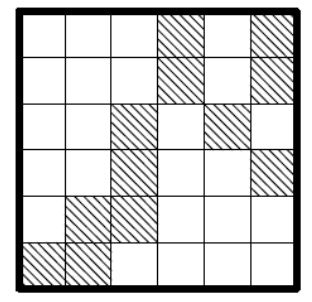
\includegraphics[width=0.2\textwidth]{pila_9.jpg}
	\end{wrapfigure}
	\textbf{№3} Разрежьте квадрат 6 × 6 на рисунке справа на 4 равные\\ части так, чтобы каждая из них содержала три закрашенные\\ клетки.
	
	\task{4} Чтобы получить 120 кг мельхиора, необходимо сплавить 18 кг никеля,\\ 24 кг цинка, а остальное - медь. Сколько килограммов каждого металла необходимо взять, чтобы получить 160 кг мельхиора?\\
	
	\task{5} Байкер в первый час проехал $\frac{3}{8}$ всего пути, во второй час $\frac{3}{5}$  остатка,\\а в третий час остальные 40 км. Найдите весь путь.\\
	
	\task{6} Найдите все целые числа, для которых выполнено равенство:\\
	\centering $|x-3|+|x+3|=6$\\ \raggedright
	
	\task{7} Лина сварила кусок мыла в форме кирпичика и использовала его 7 раз. После этого длина, ширина и высота мыла уменьшились вдвое. На сколько использований хватит оставшегося куска мыла?\\
	
	\task{8} Докажите, что на шахматной доске нельзя расставить более 8 ладей так, чтобы никакие две из них не били друг друга.\\

	\task{9} В таблице $m \times n$ расставлены числа так, что сумма чисел в любой строке равна 100,и сумма чисел в любом столбце равна 100. Докажите, что $m=n$.\\
	
	\task{10} Можно ли квадрат $10 \times 10$ разрезать на прямоугольники $1 \times 4$?\\
	
\end{document} 